% !TEX root = /home/fred-olav/afgv/src/preamble.tex
\input preamble.tex
\huge
\centerline{\bf Heldagsprøve Gand reguleringsstasjon 23/24}  \bigskip
\normalsize
\vskip 1cm 
Kompetansemål:
\begin{itemize}[noitemsep]

	\item Prøven dekker alle kompetansemål i automatiseirngsfaget fra VG1 til VG3 auto.  
\end{itemize}

Alle ark som leveres inn skal ha elevens navn. \\ 

\oppgave{}%7
% Elektroteknikk
\textbf{a)}\\
Programmer denne simuleringsfunksjonen for et temperaturreguleringssystem i et PLS program
\vskip 1cm 

$$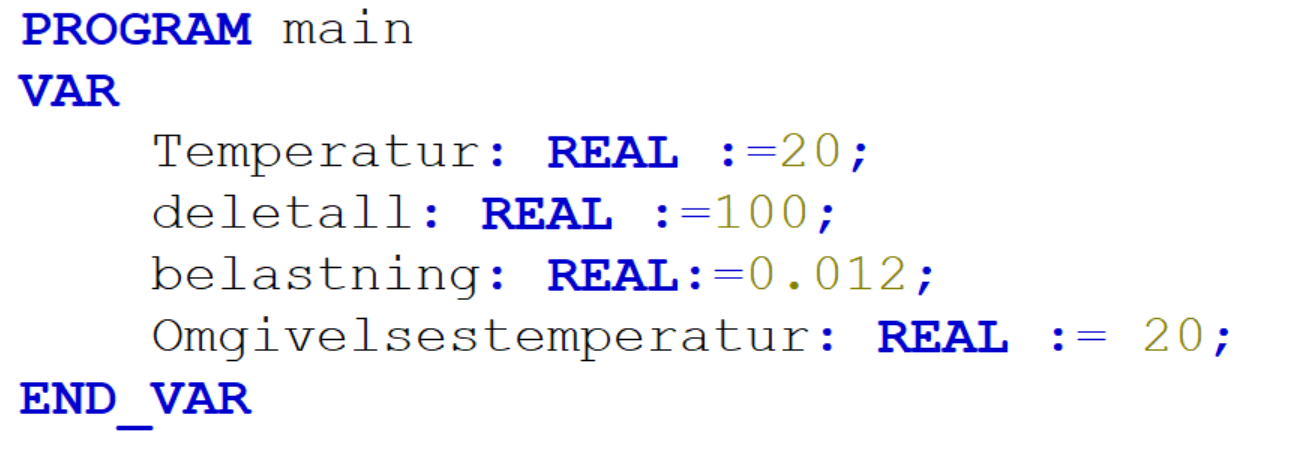
\includegraphics[width=15.5cm]{./aReg2324x05}$$
$$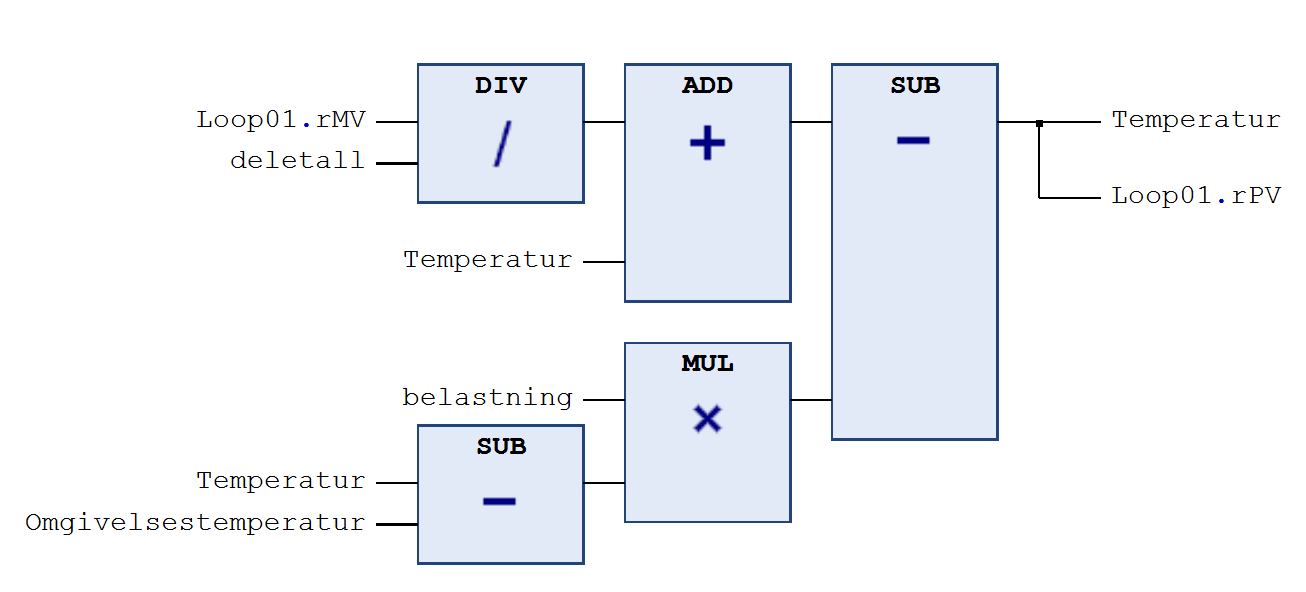
\includegraphics[width=15.5cm]{./aReg2324x06}$$

\textbf{b)}
Utvid programmet med en PID regulator som kan regulere simuleringsmodellen
\vskip 1cm 
\textbf{c)}
Programmer to skalleringsfunksjoner for temperaturtransmitter og reguleringsventil som tilkobles h.h.v. Wago 750-455 (AI 0-32760) og 750-555 (AO 0-32767). Disse to nettene skal kommenteres ut slik at de ikke er aktive i programmet. 
\vskip 1cm 
\oppgave{}%8
% Elektroteknikk
Du skal lagen HMI styring til reguleringen av den simulerte modellen av et temperaturreguleringssystem. Det skal bestå av tre bilder:
\begin{itemize}
	\item Hovedmeny
	\item L3 P \& ID "bilde" av prosessen
	\item L4 Optimaliseringsbilde av prosessen
\end{itemize}

På L3 bildet skal det byttes faceplate når en hoder musen over ventilen. 


$$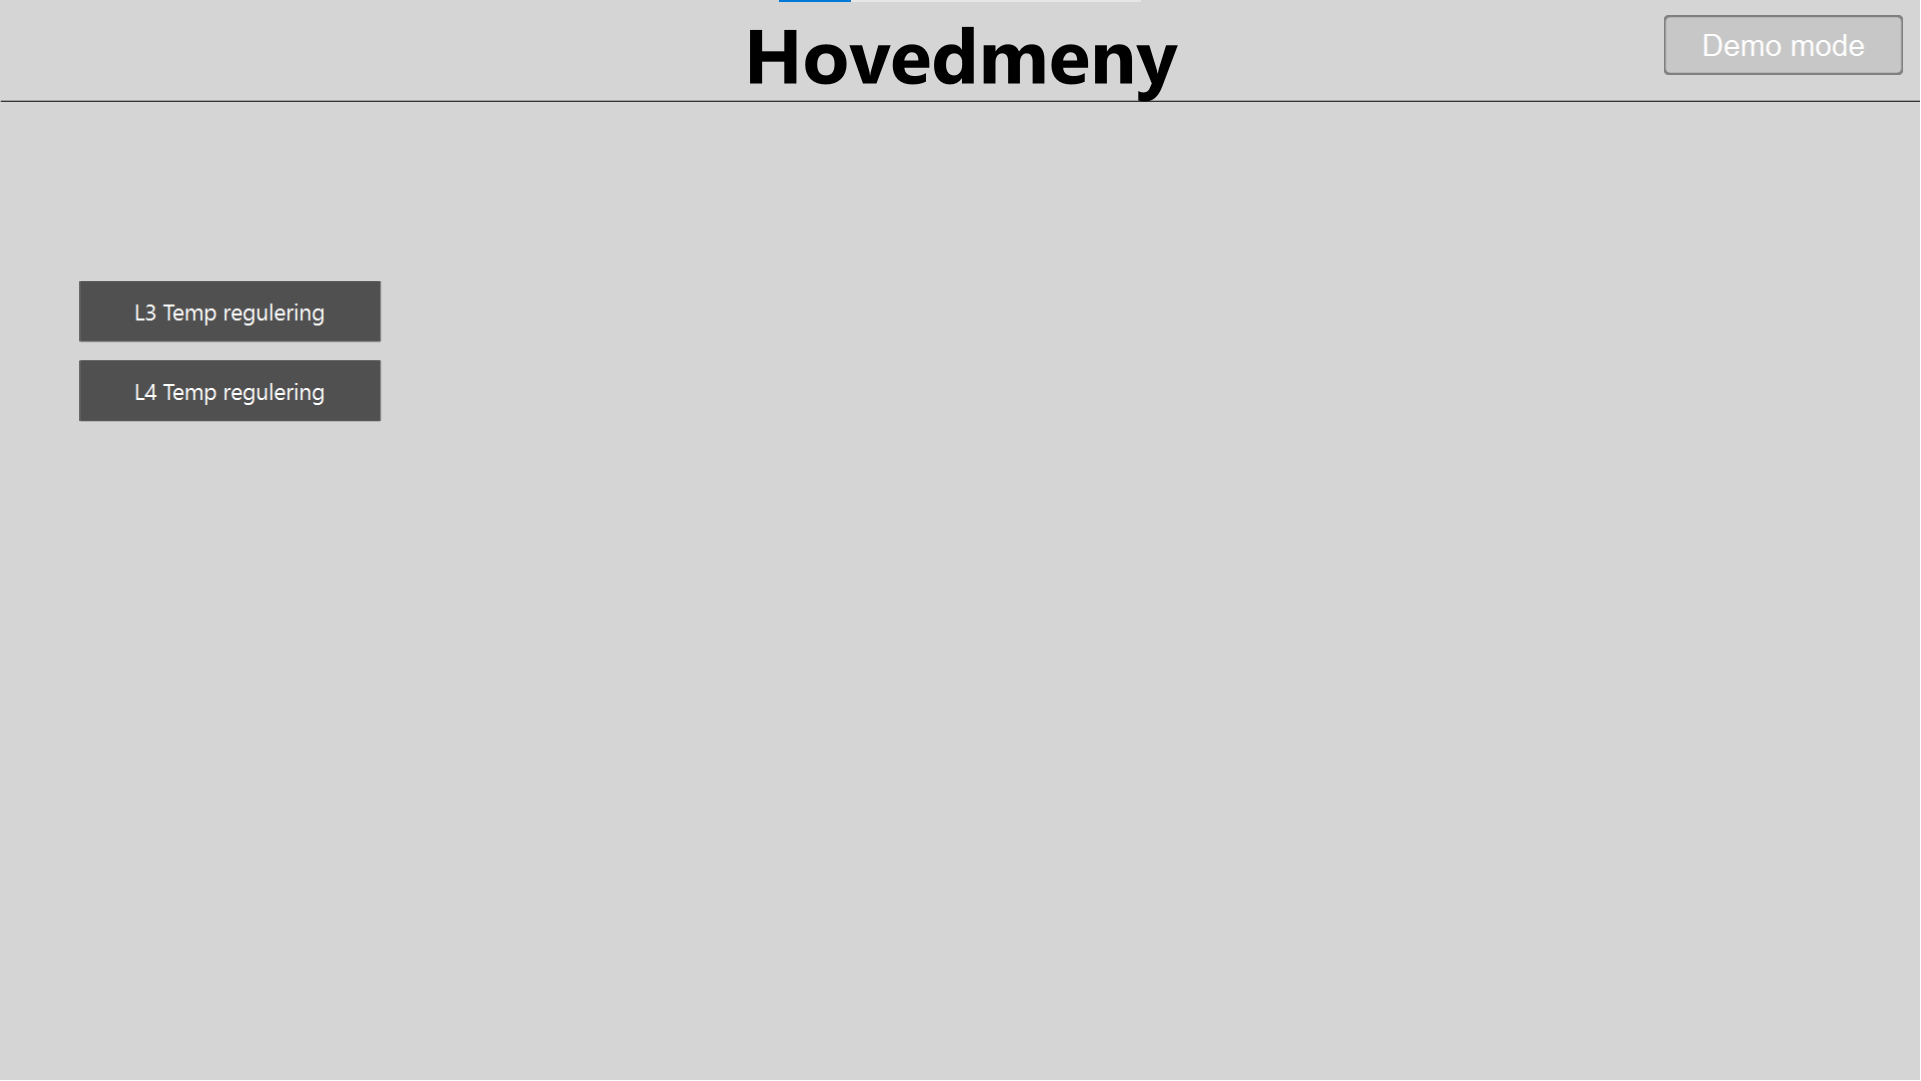
\includegraphics[width=15.5cm]{./aReg2324x03}$$
$$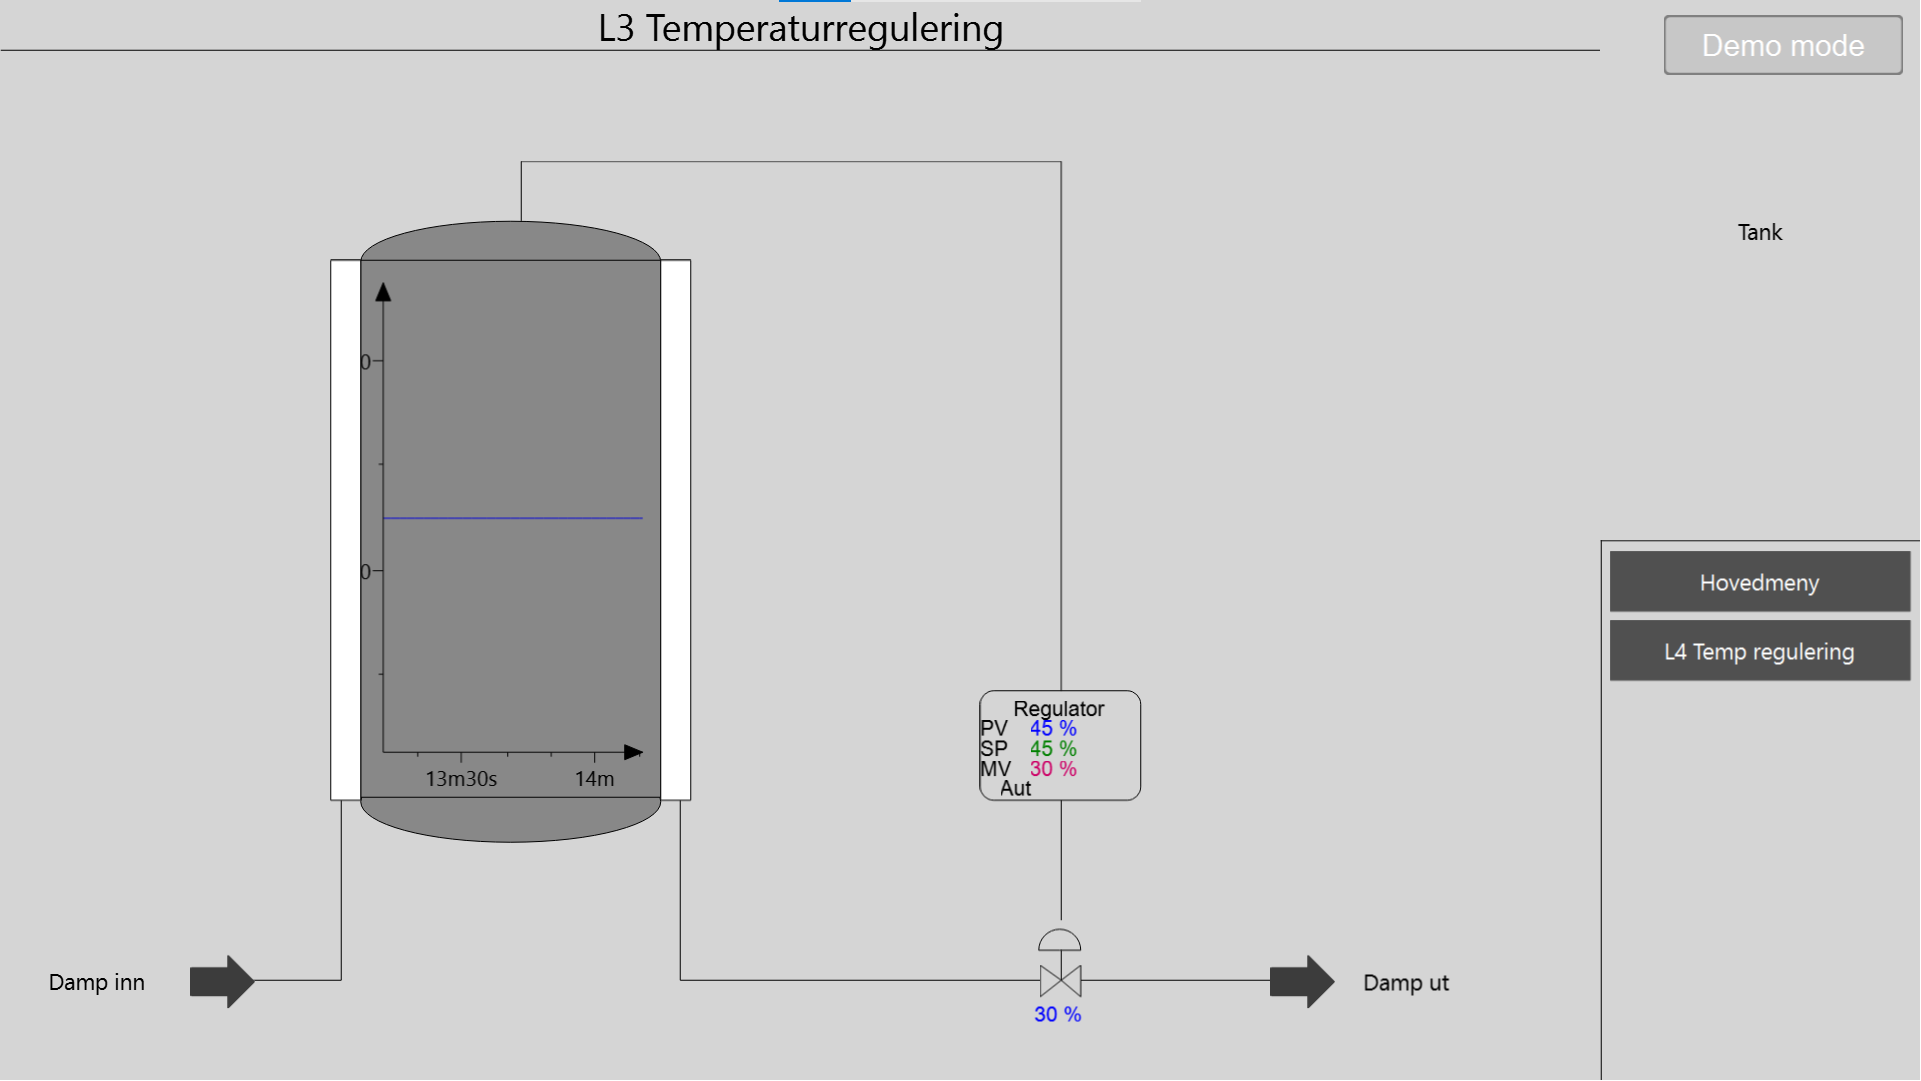
\includegraphics[width=15.5cm]{./aReg2324x02}$$

\vskip 2cm
\vfil \eject
\oppgave{}%2
% Elektroteknikk
%$$\includegraphics[width=15.5cm]{i04867x01.eps}$$


\textbf{a)}
Du skal klargjøre en målesløyfe for kalibrering. Tegn hvordan du ville koblet opp en komplett 4-20 mA målesløyfe

\vskip 1cm 

\begin{tikzpicture}
	\draw[step=0.5cm,gray!20,very thin]  grid (16,4) ;
\end{tikzpicture}
\vskip 1cm 

\textbf{b)}
Forklar (og tegn) forskjellen på 2-leder, 3-leder og 4-lederkobling av PT100-elementer.
\vskip 1cm 

\begin{tikzpicture}
	\draw[step=0.5cm,gray!20,very thin]  grid (16,4) ;
\end{tikzpicture}
\vskip 1cm 
\textbf{c)}
Gi en detaljert beskrivelse av hvordan vi kan benytte et termoelement til temperaturmåling.
\vskip 1cm 

\begin{tikzpicture}
	\draw[step=0.5cm,gray!20,very thin]  grid (16,4) ;
\end{tikzpicture}
\vskip 1cm 

\textbf{e)}
Du kontrollere en målesløyfe som inneholder et termoelement type K. Temperaturen i
kalibreringsverkstedet er nå 22°C.
\\
Du varmer målepunktet opp til 100°C. Hvilken verdi vil du måle i referansepunktet til termoelementet?
\\
Termoelementet er tilkoblet en måleomformer som gir ut 4-20 mA, og du skal kalibrere denne målesløyfen etter
5-punktsmetoden. Måleomfanget er 0-750°C. Fyll ut tabellen under på forventede (ideelle) måleverdier.

\begin{center}
	\begin{tabular}{| m{3.5cm} |m{3.5cm} |m{3.5cm} |m{3.5cm} |} 
\hline
	\multicolumn{4}{|c|}{\textbf{\cellcolor[HTML]{D5D5D5}Referansetemperatur: 22°C}} \\
\hline
\hline
\rowcolor [HTML]{D5D5D5}
		Testpunkt [\%] & Temperatur [°C]& PT100-element [$\Omega$]& Måleomformer [V]\\ 
\hline


\rule{0pt}{25pt}& & & \\   \hline
\rule{0pt}{25pt}& & & \\   \hline
\rule{0pt}{25pt}& & & \\   \hline
\rule{0pt}{25pt}& & & \\   \hline
\rule{0pt}{25pt}& & & \\   \hline
		
\end{tabular}
\end{center}

\oppgave{}%1
\textbf{a)}
Hvordan fungerer en kapasitiv nivåmåler?
\vskip 1cm 

\begin{tikzpicture}
	\draw[step=0.5cm,gray!20,very thin]  grid (16,4) ;
\end{tikzpicture}
\vskip 1cm 
\textbf{a)}
Gi en kort forklaring på hvordan måling med boblerør fungerer?
\vskip 1cm 

\begin{tikzpicture}
	\draw[step=0.5cm,gray!20,very thin]  grid (16,4) ;
\end{tikzpicture}
\vskip 1cm 





\textbf{a)}
En åpen tank (HxD = 3 x 0,5 m) er utstyrt med hydrostatisk nivåmåling ved hjelp d/p-celle. Mediet som måles er glycerin. Dette har en densistet (tetthet) på 1,26x10\textsuperscript{3} kg/m\textsuperscript{3}.\\
Du skal klargjøre d/p-cellen for benkkalibrering:\\
Hvilket trykk må du påføre på høytrykksiden og lavtrykksiden av d/p-cellen for å simulere 100 \% fyllingsgrad i tanken?
\vskip 1cm 

\begin{tikzpicture}
	\draw[step=0.5cm,gray!20,very thin]  grid (16,4) ;
\end{tikzpicture}
\vskip 1cm 

\vfil \eject
\oppgave{}%2.
\textbf{a)}\\
På reguleringsanlegget har dere montert, kalibrert, justert og igangsatt en reguleringsventil med tilhørende IP-omformer og ventilstiller. Tegn og forklar hvordan delene fungerer sammen, og hva som er «jobben» til ventilstilleren. Klarer du å forklare hvordan den gjør det er det supert.  
\vskip 1cm 

\begin{tikzpicture}
	\draw[step=0.5cm,gray!20,very thin]  grid (16,20) ;
\end{tikzpicture}
\vskip 1cm 

\vfil \eject
\oppgave{}%3
% Elektroteknikk
\textbf{a)}\\
Fokuser på flow-sløyfa på flytskjemaet under; hvilke komponenter skal plasseres hvor i blokkskjemaet til ei reguleringssløyfe? Hvilke signal blir sendt mellom de ulike delene? (tegn hele sløyfa på svar-arket, og fyll inn navnene i de ulike firkantene) 

$$\includegraphics[width=15.5cm]{../output/noGPLimages/aReg2324x07.png}$$
\vskip 1cm 

\begin{tikzpicture}
	\draw[step=0.5cm,gray!20,very thin]  grid (16,10) ;
\end{tikzpicture}
\vskip 1cm 
\textbf{b)}
Forklar hvordan hele prosessen(e) fungerer. (Tanken har et varmevekslerprinsipp, hvor dampen ikke kommer i direkte kontakt med væska.)

\vskip 1cm 

\begin{tikzpicture}
	\draw[step=0.5cm,gray!20,very thin]  grid (16,22) ;
\end{tikzpicture}
\vskip 1cm 

\vfil \eject


\vfil \eject
\oppgave{}%4
\textbf{a)}
Tegn og forklar virkemåten til strømningsmåling med måleblende
\vskip 1cm

\begin{tikzpicture}
	\draw[step=0.5cm,gray!20,very thin]  grid (16,10) ;
\end{tikzpicture}
\vskip 1cm

\textbf{b)}
Vi har et rør som det strømmer castor olje ($\mu=0.650 Pa\cdot s$ $\rho$=957kg/m³) med en strømningsrate på 185 l/s. Begge seksjonene er etter schedule 40.  Den første delen av røret har dimensjon DN200 (ID=202.74mm) og den andre delen har dimensjon DN65 (ID=62.68mm)

$$\includegraphics[width=15.5cm]{~/afgv/src/i04033x01.eps}$$

Regn ut hastigheten for fluidet i røret for hver av seksjonene. 
\vskip 1cm

\begin{tikzpicture}
	\draw[step=0.5cm,gray!20,very thin]  grid (16,5) ;
\end{tikzpicture}
\vskip 1cm


\textbf{c)}
Regn ut reynolds tall for hver av seksjonene
\vskip 1cm

\begin{tikzpicture}
	\draw[step=0.5cm,gray!20,very thin]  grid (16,5) ;
\end{tikzpicture}
\vskip 1cm
\textbf{d)}
Tegn strømingsprofilene og sett navn på
\vskip 1cm

\begin{tikzpicture}
	\draw[step=0.5cm,gray!20,very thin]  grid (16,5) ;
\end{tikzpicture}
\vskip 1cm



\newpage
$$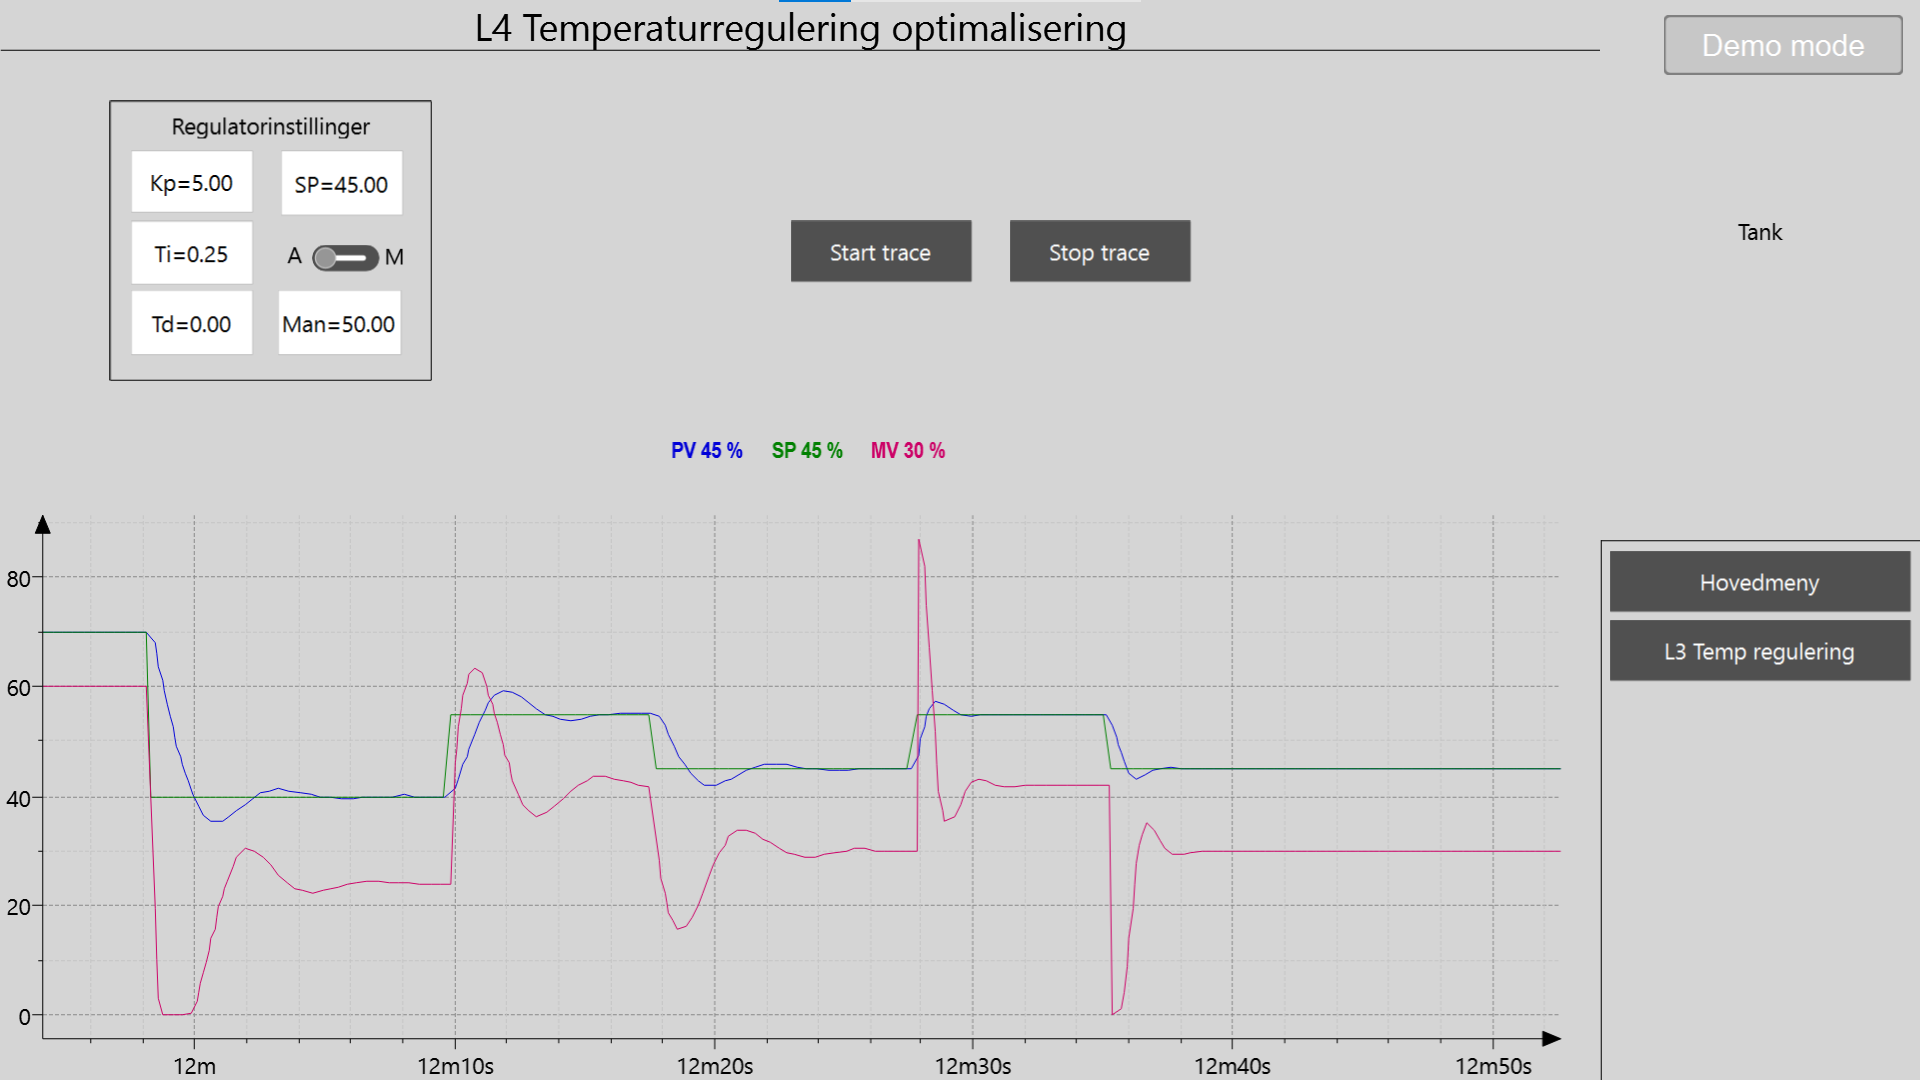
\includegraphics[width=15.5cm]{./aReg2324x01}$$
\oppgave{}%9
Vis hvordan du kan optimalisere prosessen fra forrige oppgave. Bruk screenshot for å vise alle verdier du henter fra HMI. \\
Om du ikke har noe program fra forrige oppgave må du tegne og forklare hvordan du ville gått frem. 
\vskip 2cm
\oppgave{}%9
% Elektroteknikk
Du har fått i oppdrag i å montere og koble opp (ikke programmere) et Wago TP600 (delenummer 762-5306/8000-0002, size 10") touchpanel skapdøren på Gand reguleringsstasjon. \\
Vis hvordan du ville planlagt, gjennomført og dokumentert oppdraget.
\vskip 2 cm 
Dokumentasjon på panelet sende til den epost når prøven starter. 
\includepdf[pages=-,angle=90]{../eq/afgvformler.pdf}
\end {document}
